% Provenance (never printed): old terminale S material on mountain ranges and
% continental collision (folds, reverse faults and nappes as signs of
% shortening and thickening; ophiolites and sutures as the trace of a closed
% ocean; the Himalaya and the Alps as examples). Owner (Sync 0): collision,
% fold/anticline/syncline/fold axis, reverse fault/thrust, nappe, ophiolite,
% suture, shortening. Fault is Book 1's (g7), normal fault g11.05's, the root
% and Airy isostasy g11.03's and g12.01's: recalled, never redefined. India's
% past latitudes: figdata/grade-12/india_drift.py (GPlates Web Service, two
% published plate models); shortening: figdata/grade-12/fold_shortening.py;
% the belt map: figdata/grade-12/alpine_belt.py.
\chapter{بناء الجبال}\label{ch:g12:mountain-building}

المتسلقون الذين يبلغون قمة جبل إيفرست، على ارتفاع \qty{8848.86}{m} فوق مستوى سطح
البحر، يقفون على حجر جيري. فالجيولوجيون الذين أنزلوا عينات من
القمة وجدوا فيها قطعًا مكسورة من ثلاثيات الفصوص والأوستراكودا
وزنابق البحر: كائنات بحرية عاشت قبل أكثر من 440 مليون سنة، في
الأوردوفيشي. فأعلى صخر في العالم ترسب على قاع
بحر. يشرح هذا الفصل كيف ينتهي قاع بحر على سطح العالم:
تتصادم قارتان، فتُعصر القشرة بينهما وتُطوى
وتُكدَّس وتُسمَّك حتى تصير سلسلة جبلية.
% ledger: sakai05:summit, tulane:roots (marine limestones at the top of Mt. Everest), ics:base.Ordovician, ics:base.Silurian (486.85-443.1 Ma); Book 1: tht:everest (8848.86 m)

\begin{omfigure}
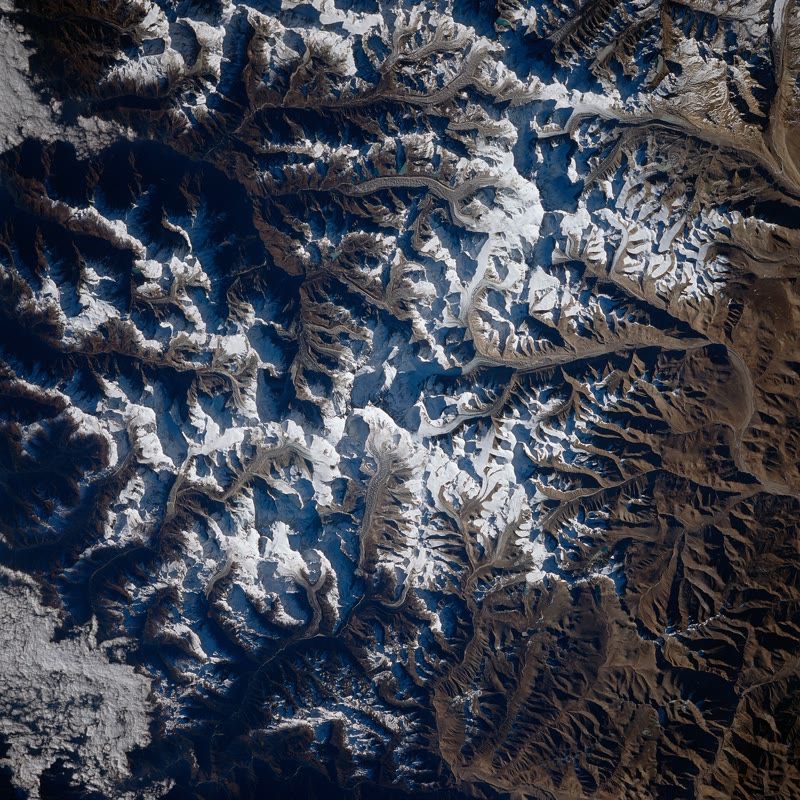
\includegraphics[width=0.5\linewidth]{images/book2/g12-nasa-everest-columbia.jpg}

{\small جبل إيفرست وأنهار جليدية كثيرة حوله، كما رُئيت من المكوك
الفضائي كولومبيا في 30 نوفمبر 1996. الصورة: ناسا (ملك عام).}
\end{omfigure}
% ledger: photo:g12-everest-columbia

\begin{recall}
صفيحة من \omterm{def:g11:ocean-ridges:oceanic-lithosphere}{الغلاف الصخري المحيطي}، تُصنع عند ظهرة، تغوص عائدة إلى الوشاح
عند خندق؛ \omterm{def:g11:subduction-zones:slab}{ولوحها المندس} يسحبها إلى الأسفل (\cref{ch:g11:subduction-zones}).
\omterm{def:g12:continental-crust:continental-crust}{والقشرة القارية} سميكة وخفيفة، نحو \qty{2830}{kg/m^3} في المتوسط
مقابل \qty{3380}{kg/m^3} للوشاح الذي تحتها، فهي تطفو عاليًا،
والقشرة السميكة تقف أعلى من الرقيقة، فوق \omterm{def:g12:continental-crust:root}{جذر}
(\cref{ch:g12:continental-crust,ch:g11:lithosphere-asthenosphere}). والصدع
كسر تحرك على امتداده الكتلتان؛ وفي \omterm{def:g11:ocean-ridges:normal-fault}{الصدع العادي} تكون
الكتلة التي فوق مستوى الصدع قد تحركت إلى الأسفل، كما حيث تتمطط القشرة
عند ظهرة بطيئة (\cref{ch:g11:ocean-ridges}).
\end{recall}
% ledger: cm95:crust, data:prem, tulane:no-subduct, usgs:normal-fault

\section{من الاندساس إلى الاصطدام}

المحيط الذي يُستهلك عند خندق أسرع مما يُصنع عند ظهرته
ينكمش. والقارة المحمولة على الصفيحة الغائصة تقترب من الخندق
بسرعة الصفيحة، وتصل إليه في النهاية. \omterm{def:g11:ocean-ridges:oceanic-lithosphere}{فالغلاف الصخري
المحيطي} الذي أمامها قد نزل؛ ولا تستطيع القارة أن تتبعه،
لأن قشرتها أخف من أن تغوص في الوشاح الأكثف. فيتوقف
\omterm{def:g11:subduction-zones:subduction}{الاندساس}. وتُعصر القارتان إحداهما على الأخرى، \omterm{def:g11:subduction-zones:slab}{واللوح المندس}
الذي كان متدليًا من قاع المحيط ينفصل في النهاية ويغوص في
الوشاح.
% ledger: earle:collision, tulane:no-subduct

\begin{definition}[الاصطدام القاري]\label{def:g12:mountain-building:collision}
\emph{الاصطدام القاري}\index{اصطدام قاري} هو التقاء
قارتين عند حد صفائح متقارب، بعد أن يندس \omterm{def:g11:ocean-ridges:oceanic-lithosphere}{الغلاف الصخري المحيطي}
الذي بينهما. ولا تغوص أي من القارتين: فالقشرة التي بينهما
تتشوه وتُسمَّك حتى تصير حزامًا جبليًا.
\end{definition}
% ledger: earle:collision, tulane:no-subduct, usgs:himalaya-collision

\begin{omfigure}
\begin{tikzpicture}[x=0.95cm, y=0.95cm, font=\scriptsize]
  % ---- stage 1: the ocean closes ----
  \begin{scope}[yshift=0cm]
    \fill[omSea] (3.4,0) -- (8.6,0) -- (8.0,-0.5) -- (4.3,-0.5) -- (3.5,0.0) -- cycle;
    \fill[omLithGranite] (0,0.15) -- (3.5,0.15) -- (4.3,-0.5) -- (4.3,-0.75) -- (3.5,-1.0) -- (0,-1.0) -- cycle;
    \fill[omLithBasalt] (4.3,-0.5) -- (8.0,-0.5) .. controls (9.0,-0.75) and (9.6,-1.2) .. (10.4,-2.0)
      -- (10.15,-2.15) .. controls (9.4,-1.4) and (8.9,-1.0) .. (8.0,-0.75) -- (4.3,-0.75) -- cycle;
    \fill[omLithGranite] (8.0,-0.5) -- (8.6,0.2) -- (12,0.2) -- (12,-1.05) -- (9.5,-1.05)
      .. controls (9.0,-0.75) .. (8.0,-0.5) -- cycle;
    \fill[omThm!70] (10.0,0.2) -- (10.3,0.55) -- (10.6,0.2) -- cycle;
    \draw[black!60, line width=0.3pt] (0,0.15) -- (3.5,0.15) -- (4.3,-0.5) -- (8.0,-0.5) -- (8.6,0.2) -- (12,0.2);
    \draw[-{Stealth[length=2mm]}, line width=0.8pt] (1.2,0.45) -- (2.6,0.45);
    \node[anchor=east] at (0,-0.4) {1};
    \node at (1.8,-0.5) {قارة};
    \node at (6.1,-0.25) {محيط};
    \node[anchor=north] at (6.1,-0.8) {غلاف صخري محيطي};
    \node[anchor=south] at (8.0,0.0) {خندق};
    \node[anchor=south] at (10.3,0.55) {قوس بركاني};
    \node at (11.1,-0.5) {قارة};
  \end{scope}
  % ---- stage 2: the continents meet ----
  \begin{scope}[yshift=-3.0cm]
    \fill[omSea] (6.9,0) -- (8.4,0) -- (8.0,-0.4) -- (7.4,-0.35) -- cycle;
    \fill[omLithGranite] (0,0.15) -- (6.8,0.15) -- (7.6,-0.4) -- (8.0,-0.5)
      .. controls (9.0,-0.75) .. (9.5,-1.05) -- (9.2,-1.4) -- (6.5,-1.0) -- (0,-1.0) -- cycle;
    \fill[omLithBasalt] (9.5,-1.05) .. controls (10.0,-1.4) .. (10.6,-2.0) -- (10.35,-2.15)
      .. controls (9.8,-1.6) .. (9.2,-1.4) -- cycle;
    \fill[omLithGranite] (8.0,-0.5) -- (8.6,0.2) -- (12,0.2) -- (12,-1.05) -- (9.5,-1.05)
      .. controls (9.0,-0.75) .. (8.0,-0.5) -- cycle;
    \fill[omLithPeridotite] (7.0,0.15) -- (7.9,0.15) -- (8.3,0.05) -- (7.95,-0.12) -- (7.3,0.0) -- cycle;
    \fill[omThm!70] (10.0,0.2) -- (10.3,0.55) -- (10.6,0.2) -- cycle;
    \draw[-{Stealth[length=2mm]}, line width=0.8pt] (3.2,0.45) -- (4.6,0.45);
    \node[anchor=east] at (0,-0.4) {2};
    \node at (3.4,-0.45) {قارة};
    \draw[black!60] (7.6,0.12) -- (7.0,0.75) node[anchor=south east, inner sep=1pt] {شريحة من قاع المحيط};
    \node at (11.1,-0.5) {قارة};
    \node[anchor=west] at (10.7,-1.9) {لوح مندس};
  \end{scope}
  % ---- stage 3: a mountain belt ----
  \begin{scope}[yshift=-6.4cm]
    \fill[omLithGranite] (0,0.15) -- (4.5,0.15) .. controls (6.0,0.4) and (6.6,1.25) .. (7.6,1.3)
      .. controls (8.7,1.3) and (9.6,0.5) .. (10.6,0.2) -- (12,0.2) -- (12,-1.05) -- (10.6,-1.1)
      .. controls (9.5,-2.2) and (8.6,-2.6) .. (7.7,-2.6) .. controls (6.6,-2.6) and (5.6,-1.6) .. (4.5,-1.0)
      -- (0,-1.0) -- cycle;
    \draw[black!60, line width=0.3pt] (0,0.15) -- (4.5,0.15) .. controls (6.0,0.4) and (6.6,1.25) .. (7.6,1.3)
      .. controls (8.7,1.3) and (9.6,0.5) .. (10.6,0.2) -- (12,0.2);
    \draw[black!60, dashed, line width=0.4pt] (0,-1.0) -- (4.5,-1.0) .. controls (5.6,-1.6) and (6.6,-2.6) .. (7.7,-2.6)
      .. controls (8.6,-2.6) and (9.5,-2.2) .. (10.6,-1.1) -- (12,-1.05);
    \draw[omThm, line width=1.0pt] (7.0,1.25) -- (8.3,-2.55);
    \foreach \t in {0.15,0.4,0.65}
      \fill[omLithPeridotite] ($(7.0,1.25)!\t!(8.3,-2.55)$) ++(-0.12,0.05) -- ++(0.3,0) -- ++(-0.05,-0.22) -- ++(-0.3,0) -- cycle;
    \fill[omLithBasalt] (10.9,-1.9) -- (11.5,-2.35) -- (11.35,-2.5) -- (10.75,-2.05) -- cycle;
    \node[anchor=east] at (0,-0.4) {3};
    \node at (2.4,-0.45) {قارة};
    \node at (11.3,-0.5) {قارة};
    \draw[black!60] (7.2,0.6) -- (5.9,1.5) node[anchor=east, inner sep=1pt] {درز وأوفيوليتات};
    \node at (7.7,-1.9) {جذر};
    \node[anchor=north] at (11.2,-2.5) {لوح مندس منفصل};
    \node[anchor=south] at (7.6,1.35) {حزام جبلي};
  \end{scope}
\end{tikzpicture}

{\small من \omterm{def:g11:subduction-zones:subduction}{الاندساس} إلى الاصطدام (رسم، ليس بمقياس رسم حقيقي). 1: يُغلق محيط إذ
يغوص قاعه عند خندق. 2: تصل القارة إلى الخندق ولا
تستطيع أن تغوص؛ فتُدفع شرائح من قاع المحيط على حافتها. 3: تُقصَّر القشرة
الواقعة بين القارتين وتُسمَّك حتى تصير حزامًا جبليًا
قائمًا فوق \omterm{def:g12:continental-crust:root}{جذر}؛ والخط الذي التحمت عنده القارتان، والذي تدل عليه
شرائح من قاع المحيط، هو \omterm{def:g12:mountain-building:suture}{الدرز}؛ وينفصل \omterm{def:g11:subduction-zones:slab}{اللوح المندس} ويغوص.}
\end{omfigure}
% ledger: earle:collision, tulane:ocean-basins, usgs:suture, tulane:roots

\subsection{أثر محيط زائل}

حين يُغلق المحيط، تلتحم القارتان على امتداد خط.

\begin{definition}[الدرز]\label{def:g12:mountain-building:suture}
\emph{الدرز}\index{درز} هو الخط، أو النطاق الضيق، الذي التحمت على امتداده
قارتان باصطدام، بعد أن توقف \omterm{def:g11:subduction-zones:subduction}{الاندساس} بينهما:
وهو أثر حد صفائح سابق. ويدل على المكان الذي كان فيه المحيط
الذي بينهما.
\end{definition}
% ledger: usgs:suture, liu20:itsz

ما الذي يدل على \omterm{def:g12:mountain-building:suture}{الدرز}؟ على امتداد كثير من الدروز تقع أجسام صخرية لا تنتمي
إلى أي مكان في قارة: فمن الأعلى إلى الأسفل، رسوبيات بحرية، وبازلت
وسائدي، وكتلة من \omterm{def:g11:igneous-rocks:intrusion}{القواطع} الرأسية المتراصة جنبًا إلى جنب، \omterm{def:g11:ocean-ridges:gabbro}{وغابرو}، وفي
القاعدة \omterm{def:g11:ocean-ridges:peridotite}{بيريدوتيت} الوشاح: إنها طبقات قاع المحيط
(\cref{ch:g11:ocean-ridges})، وتحتها أعلى الوشاح.
% ledger: tulane:ocean-basins

\begin{definition}[الأوفيوليت]\label{def:g12:mountain-building:ophiolite}
\emph{الأوفيوليت}\index{أوفيوليت} قطعة من \omterm{def:g11:ocean-ridges:oceanic-lithosphere}{الغلاف الصخري المحيطي} ---
رسوبيات، وبازلت وسائدي، \omterm{def:g11:igneous-rocks:intrusion}{وقواطع} متراصة، \omterm{def:g11:ocean-ridges:gabbro}{وغابرو}، \omterm{def:g11:ocean-ridges:peridotite}{وبيريدوتيت} الوشاح ---
دُفعت فوق \omterm{def:g12:continental-crust:continental-crust}{قشرة قارية}.
\end{definition}
% ledger: tulane:ocean-basins

\omterm{def:g12:mountain-building:ophiolite}{الأوفيوليت} قاع محيط جانح: شريحة من المحيط الزائل، دُفعت
فوق قارة بدل أن تغوص مع الباقي. والجبال التي يرفعها
الاصطدام تحوي عادةً شيئًا من \omterm{def:g11:ocean-ridges:oceanic-lithosphere}{القشرة المحيطية} والوشاح العلوي، لأن ذلك هو
المكان الذي أُغلق فيه محيط. ففي جنوب التبت، \omterm{def:g12:mountain-building:ophiolite}{الأوفيوليتات} المنتظمة
على امتداد \omterm{def:g12:mountain-building:suture}{درز} السند--تسانغبو بقايا محيط يُسمّى
التيثس الجديد، كان يقع بين الهند ومنطقة لاسا؛ وقد أُرِّخ \omterm{def:g11:ocean-ridges:gabbro}{غابرو} هناك
فكان عمره 243 مليون سنة.
% ledger: tulane:ocean-basins, earle:collision, liu20:itsz

\begin{omfigure}
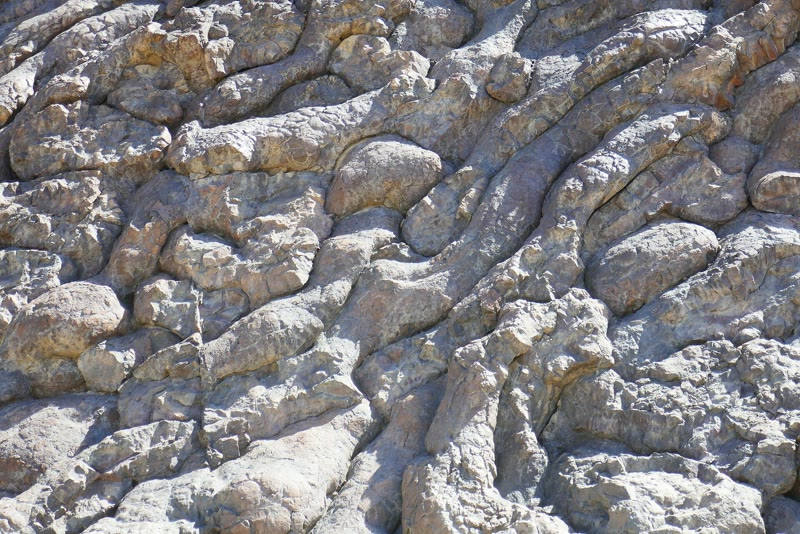
\includegraphics[width=0.6\linewidth]{images/book2/g12-duchoiselle-oman-pillows.jpg}

{\small لابة وسائدية من \omterm{def:g12:mountain-building:ophiolite}{أوفيوليت} سمائل في وادي الجزي، عُمان: لابة
بردت تحت الماء على هيئة وسائد مستديرة، وهي الآن على اليابسة. الصورة: ليونيل
دوشوازيل (\babelsublr{CC~BY-SA~3.0}).}
\end{omfigure}
% ledger: photo:g12-oman-pillows

\section{تقصير القشرة}

إذا عُصر جسم صخري من الجانبين انكسر إن كان باردًا هشًا؛ وإن
كان دافئًا بما يكفي ليسلك سلوكًا لدنًا، انطوى. والحزام الجبلي
مليء \omterm{def:g12:mountain-building:fold}{بالطيات} والصدوع معًا.
% ledger: earle:folds

\subsection{الطيات}

\begin{definition}[الطية؛ الطية المحدبة؛ الطية المقعرة؛ محور الطية]\label{def:g12:mountain-building:fold}
\emph{الطية}\index{طية} انثناء في طبقات الصخر. وجانباها المائلان
هما \emph{الجناحان}؛ ويلتقيان عند \emph{المفصل}، حيث تبلغ الطبقات أقصى
انحنائها، والخط الممتد على المفصل هو
\emph{محور الطية}\index{محور الطية}. و\emph{الطية المحدبة}\index{طية محدبة} طية تنثني طبقاتها
إلى الأعلى، ويميل جناحاها بعيدًا عن المحور؛
و\emph{الطية المقعرة}\index{طية مقعرة} طية تنثني طبقاتها إلى الأسفل، ويميل
جناحاها نحو المحور.
\end{definition}
% ledger: earle:folds, tulane:fold-geometry

المستوى المار بمفاصل الطبقات المتتالية هو المستوى المحوري.
وتأتي \omterm{def:g12:mountain-building:fold}{الطيات} المحدبة والمقعرة عادةً أزواجًا، فجناح إحداها هو
جناح التالية. \omterm{def:g12:mountain-building:fold}{والطيات} بكل الأحجام، من المجهرية إلى عشرات
الكيلومترات عرضًا. وما إن تتآكل \omterm{def:g12:mountain-building:fold}{الطية المحدبة} حتى تُظهر أقدم طبقاتها في
لبّها، وتُظهر \omterm{def:g12:mountain-building:fold}{الطية المقعرة} أحدثها؛ \omterm{def:g12:mountain-building:fold}{والطية المحدبة} ليست بالضرورة
مرتفعًا، ولا \omterm{def:g12:mountain-building:fold}{الطية المقعرة} واديًا، لأن التعرية تتبع الطبقات الصلبة
والطرية لا شكل \omterm{def:g12:mountain-building:fold}{الطية}.
% ledger: earle:folds, tulane:fold-geometry

\begin{omfigure}
\begin{tikzpicture}[x=1.2cm, y=1.2cm, font=\scriptsize]
  \def\W{6}\def\H{2.0}\def\dx{1.35}\def\dy{0.78}
  \tikzset{declare function={zb(\x,\c)=\c+0.8*cos(60*(\x-1.5));}}
  \colorlet{bandA}{omLithSchist!70}\colorlet{bandB}{omLithSand}\colorlet{bandC}{omLithShale}
  \colorlet{bandD}{icsJurassic!35}\colorlet{bandE}{icsTriassic!35}\colorlet{bandF}{icsCretaceous!45}
  % front face
  \begin{scope}
    \clip (0,0) rectangle (\W,\H);
    \fill[bandA] (0,0) rectangle (\W,\H);
    \foreach \c/\col in {0.0/bandB, 0.6/bandC, 1.2/bandD, 1.8/bandE, 2.4/bandF}
      \fill[\col] plot[domain=0:\W, samples=80, smooth] (\x,{zb(\x,\c)}) -- (\W,4) -- (0,4) -- cycle;
    \foreach \c in {0.0,0.6,1.2,1.8,2.4}
      \draw[black!55, line width=0.35pt] plot[domain=0:\W, samples=80, smooth] (\x,{zb(\x,\c)});
  \end{scope}
  % top face: outcrop bands (crossings of the top surface computed for these curves)
  \fill[bandE] (0,\H) -- (0.242,\H) -- ++(\dx,\dy) -- (\dx,\H+\dy) -- cycle;
  \fill[bandD] (0.242,\H) -- (2.758,\H) -- ++(\dx,\dy) -- (0.242+\dx,\H+\dy) -- cycle;
  \fill[bandE] (2.758,\H) -- (3.5,\H) -- ++(\dx,\dy) -- (2.758+\dx,\H+\dy) -- cycle;
  \fill[bandF] (3.5,\H) -- (5.5,\H) -- ++(\dx,\dy) -- (3.5+\dx,\H+\dy) -- cycle;
  \fill[bandE] (5.5,\H) -- (\W,\H) -- ++(\dx,\dy) -- (5.5+\dx,\H+\dy) -- cycle;
  \foreach \x in {0.242,2.758,3.5,5.5} \draw[black!55, line width=0.35pt] (\x,\H) -- ++(\dx,\dy);
  % right face: the layers meet it at constant heights (cylindrical folds)
  \foreach \lo/\hi/\col in {0.0/0.6/bandB, 0.6/1.2/bandC, 1.2/1.8/bandD, 1.8/2.0/bandE}
    \fill[\col] (\W,\lo) -- (\W+\dx,\lo+\dy) -- (\W+\dx,\hi+\dy) -- (\W,\hi) -- cycle;
  \foreach \y in {0.6,1.2,1.8} \draw[black!55, line width=0.35pt] (\W,\y) -- ++(\dx,\dy);
  % outline
  \draw[black, line width=0.5pt] (0,0) rectangle (\W,\H) (0,\H) -- (\dx,\H+\dy) -- (\W+\dx,\H+\dy) -- (\W,\H)
    (\W+\dx,\H+\dy) -- (\W+\dx,\dy) -- (\W,0);
  % fold axes on the top face, axial planes on the front face
  \draw[omThm, line width=1pt] (1.5,\H) -- ++(\dx,\dy);
  \draw[omDef, line width=1pt] (4.5,\H) -- ++(\dx,\dy);
  \draw[omThm, dashed, line width=0.6pt] (1.5,0) -- (1.5,\H);
  \draw[omDef, dashed, line width=0.6pt] (4.5,0) -- (4.5,\H);
  \node[anchor=south, omThm] at (1.5+\dx,\H+\dy) {\foreignlanguage{arabic}{الطية المحدبة: محور الطية}};
  \node[anchor=south, omDef] at (4.5+\dx,\H+\dy) {\foreignlanguage{arabic}{الطية المقعرة: محور الطية}};
  \draw[black!70] (3.2,0.95) -- (3.9,-0.35) node[anchor=north] {جناح};
  \draw[black!70] (1.5,1.4) circle (0.07) -- (0.4,-0.35) node[anchor=north] {مفصل};
  \draw[black!70] (1.5,0.25) -- (2.0,-0.35) node[anchor=north] {المستوى المحوري};
\end{tikzpicture}

{\small \omterm{def:g12:mountain-building:fold}{طية محدبة} \omterm{def:g12:mountain-building:fold}{وطية مقعرة}، يقطعهما سطح تعرية مستوٍ (مخطط
كتلي، ليس بمقياس رسم حقيقي). تمتد محاور \omterm{def:g12:mountain-building:fold}{الطيات} على المفاصل؛ والخطوط
المتقطعة آثار المستويات المحورية. وعلى السطح العلوي تُظهر \omterm{def:g12:mountain-building:fold}{الطية المحدبة}
المتآكلة طبقات أقدم في لبّها، \omterm{def:g12:mountain-building:fold}{والطية المقعرة} طبقات أحدث.}
\end{omfigure}
% ledger: earle:folds, tulane:fold-geometry

\begin{omfigure}
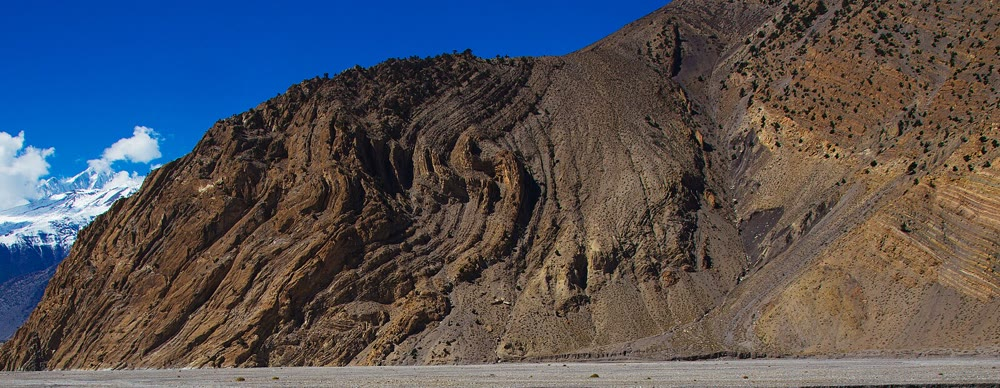
\includegraphics[width=0.95\linewidth]{images/book2/g12-hullot-kali-gandaki-folds.jpg}

{\small طبقات صخرية مطوية في جرف من الهيمالايا، على بعد نحو
\qty{3}{km} شمال شرق جومسوم في خانق كالي غانداكي، نيبال.
الصورة: جان-ماري أولو (\babelsublr{CC~BY~2.0}).}
\end{omfigure}
% ledger: photo:g12-kali-gandaki

غطاء تلال فاردن الرسوبي مطوي على النحو نفسه، لكن بلطف أكبر بكثير.
فحجره الرملي وحجره الجيري وسجيله وطباشيره ترسبت مستوية، ثم انثنت
إلى \omterm{def:g12:mountain-building:fold}{طية محدبة} \omterm{def:g12:mountain-building:fold}{وطية مقعرة} يميل جناحاهما \ang{12}؛ ثم قطعها
\omterm{def:g11:ocean-ridges:normal-fault}{صدع عادي} لاحق.
% ledger: region:name; model in figdata/shared/region.py (LIMB_DIP 12, AXIS_ANTI 3.5 km, AXIS_SYN 7.5 km)

\begin{omfigure}
\begin{tikzpicture}
\begin{axis}[omsection, x=1.25cm, y=0.003125cm, xmin=0, xmax=9.49, ymin=-700, ymax=650,
  xlabel={\foreignlanguage{arabic}{المسافة من A \babelsublr{(\unit{km})}}}, ylabel={\foreignlanguage{arabic}{الارتفاع \babelsublr{(\unit{m})}}},
  ytick={-600,-300,0,300,600}, tick label style={font=\scriptsize}]
\addplot[fill=black!8, draw=black!50, line width=0.3pt, even odd rule] table {figdata/out/shared-region-section-unit-schist.dat};
\addplot[fill=icsTriassic!20, draw=black!50, line width=0.3pt, even odd rule] table {figdata/out/shared-region-section-unit-sandstone.dat};
\addplot[fill=icsJurassic!25, draw=black!50, line width=0.3pt, even odd rule] table {figdata/out/shared-region-section-unit-limestone.dat};
\addplot[fill=icsJurassic!8, draw=black!50, line width=0.3pt, even odd rule] table {figdata/out/shared-region-section-unit-shale.dat};
\addplot[fill=icsCretaceous!20, draw=black!50, line width=0.3pt, even odd rule] table {figdata/out/shared-region-section-unit-chalk.dat};
\addplot[fill=omLithAlluv, draw=black!50, line width=0.3pt, even odd rule] table {figdata/out/shared-region-section-unit-alluvium.dat};
\addplot[black, line width=0.7pt] table {figdata/out/shared-region-section-ground.dat};
\addplot[fault] table {figdata/out/shared-region-section-fault.dat};
% axis positions from figdata/grade-12/fold_shortening.py (section_anticline_km, section_syncline_km; the syncline lies on the hanging wall, shifted by the fault heave)
\draw[omThm, dashed, line width=0.7pt] (axis cs:3.162,-700) -- (axis cs:3.162,660);
\draw[omDef, dashed, line width=0.7pt] (axis cs:7.484,-700) -- (axis cs:7.484,660);
\node[anchor=south, omThm, font=\scriptsize] at (axis cs:3.162,660) {محور الطية المحدبة};
\node[anchor=south, omDef, font=\scriptsize] at (axis cs:7.484,660) {محور الطية المقعرة};
\node[anchor=south east, font=\small\bfseries] at (axis cs:0,650) {A};
\node[anchor=south west, font=\small\bfseries] at (axis cs:9.49,650) {B};
\node[font=\scriptsize, fill=white, inner sep=1pt] at (axis cs:1.2,-520) {شيست};
\node[font=\scriptsize, fill=white, inner sep=1pt, anchor=east] at (axis cs:6.55,-450) {صدع عادي};
\end{axis}
\end{tikzpicture}

\smallskip
{\small\tikz\fill[black!8, draw=black!50] (0,0) rectangle (0.35,0.22);~شيست \quad
\tikz\fill[icsTriassic!20, draw=black!50] (0,0) rectangle (0.35,0.22);~حجر رملي \quad
\tikz\fill[icsJurassic!25, draw=black!50] (0,0) rectangle (0.35,0.22);~حجر جيري \quad
\tikz\fill[icsJurassic!8, draw=black!50] (0,0) rectangle (0.35,0.22);~سجيل \quad
\tikz\fill[icsCretaceous!20, draw=black!50] (0,0) rectangle (0.35,0.22);~طباشير \quad
\omve{2.5}}

{\small المقطع A--B عبر تلال فاردن، من الجنوب الغربي إلى
الشمال الشرقي. يستقر الغطاء الرسوبي على قاعدة الشيست وهو مطوي إلى
\omterm{def:g12:mountain-building:fold}{طية محدبة} \omterm{def:g12:mountain-building:fold}{وطية مقعرة}؛ \omterm{def:g11:ocean-ridges:normal-fault}{والصدع العادي}، الأحدث من \omterm{def:g12:mountain-building:fold}{الطيات}، يُهبط
الكتلة الشمالية الشرقية. والمقياس الرأسي مُمطَّط 2.5 مرة، وهذا
يجعل الجناحين يبدوان أشد ميلًا مما هما. البيانات: نموذج السلسلة
للمنطقة.}
\end{omfigure}
% ledger: region:name; computed in figdata/shared/region.py (section A-B)

\subsection{الصدوع المعكوسة والصدوع الزاحفة والأغطية التكتونية}

حيث تُعصر القشرة وهي باردة هشة، تنكسر على امتداد صدوع
من نوع آخر غير \omterm{def:g11:ocean-ridges:normal-fault}{الصدوع العادية} في القشرة المتمططة.

\begin{definition}[الصدع المعكوس؛ الصدع الزاحف]\label{def:g12:mountain-building:thrust}
\emph{الصدع المعكوس}\index{صدع معكوس} صدع مائل تحركت على امتداده
الكتلة التي فوق مستوى الصدع إلى الأعلى بالنسبة إلى الكتلة التي
تحته. وتتكوّن الصدوع المعكوسة حيث تُعصر القشرة.
و\emph{الصدع الزاحف}\index{صدع زاحف} صدع معكوس ميله خفيف، أقل من
\ang{45}.
\end{definition}
% ledger: earle:reverse-thrust, tulane:fold-geometry

يستطيع \omterm{def:g12:mountain-building:thrust}{الصدع الزاحف} أن يحمل صفيحة من الصخر عشرات الكيلومترات، فتستقر عندئذ صخور
أقدم فوق صخور أحدث، خلافًا للترتيب الذي
ترسبت به. ففي جبال روكي، دفع \omterm{def:g12:mountain-building:thrust}{صدع ماكونيل الزاحف}
كومة من الصخور الرسوبية سمكها نحو \qty{800}{m} مسافة نحو \qty{40}{km} من
الغرب إلى الشرق: فحجر جيري عمره نحو 500 مليون سنة يستقر الآن على حجر طيني
عمره نحو 75 مليون سنة.
% ledger: earle:reverse-thrust

\begin{definition}[الغطاء التكتوني]\label{def:g12:mountain-building:nappe}
\emph{الغطاء التكتوني}\index{غطاء تكتوني} صفيحة كبيرة من الصخر حُملت
مسافة طويلة، كثيرًا ما تبلغ عشرات الكيلومترات، فوق الصخور التي تحتها على امتداد
\omterm{def:g12:mountain-building:thrust}{صدع زاحف} يكاد يكون مستويًا.
\end{definition}
% ledger: ngu:nappe, earle:reverse-thrust

قد يحمل \omterm{def:g12:mountain-building:nappe}{الغطاء التكتوني} صخورًا تكوّنت بعيدًا، بل شرائح من قاع المحيط؛ وقد
يكون هو نفسه مطويًا، وطبقاته مقلوبة. والأحزمة الجبلية تكدّس الأغطية
بعضها فوق بعض. ثم تحفر التعرية ثقوبًا في الغطاء، فتفتح
نوافذ على الصخور التي تحته، وتترك منه قطعًا معزولة قائمة على
الصخور الأحدث.
% ledger: ngu:nappe

\begin{omfigure}
\begin{tikzpicture}[x=1.0cm, y=1.0cm, font=\scriptsize]
  % rocks in place (younger), flat-lying
  \fill[icsCretaceous!25] (0,-1.6) rectangle (12,-0.4);
  \fill[icsJurassic!25] (0,-1.6) rectangle (12,-1.1);
  \draw[black!50, line width=0.3pt] (0,-1.1) -- (12,-1.1);
  \fill[white] (5.6,-0.4) -- (6.2,-0.62) -- (6.8,-0.4) -- cycle;
  % the nappe (older rocks) above a nearly flat thrust, cut by erosion
  \fill[omLithSchist!80] (0.8,-0.4) .. controls (1.2,0.35) and (1.9,0.35) .. (2.3,-0.4) -- cycle;
  \fill[omLithSchist!80] (3.2,-0.4) .. controls (3.9,0.9) and (4.8,0.9) .. (5.6,-0.4) -- cycle;
  \fill[omLithSchist!80] (6.8,-0.4) .. controls (7.1,0.9) and (7.7,1.3) .. (8.4,1.25) -- (12,0.9) -- (12,-0.4) -- cycle;
  % ground surface
  \draw[black, line width=0.6pt] (0,-0.4) -- (0.8,-0.4) .. controls (1.2,0.35) and (1.9,0.35) .. (2.3,-0.4)
     -- (3.2,-0.4) .. controls (3.9,0.9) and (4.8,0.9) .. (5.6,-0.4) -- (6.2,-0.62) -- (6.8,-0.4)
     .. controls (7.1,0.9) and (7.7,1.3) .. (8.4,1.25) -- (12,0.9);
  % thrust traces (teeth on the block that moved over)
  \draw[thrust fault] (0.8,-0.4) -- (2.3,-0.4);
  \draw[thrust fault] (3.2,-0.4) -- (5.6,-0.4);
  \draw[thrust fault] (6.8,-0.4) -- (12,-0.4);
  \draw[-{Stealth[length=2mm]}, line width=0.9pt] (11.4,1.45) -- (9.6,1.6);
  \node[anchor=south] at (10.5,1.55) {حركة الغطاء التكتوني};
  \node at (9.9,0.3) {\foreignlanguage{arabic}{الغطاء: صخور أقدم}};
  \node[fill=white, inner sep=1pt] at (2.0,-0.85) {\foreignlanguage{arabic}{صخور في مكانها: أحدث}};
  \draw[black!60] (1.55,0.0) -- (1.3,0.8) node[anchor=south] {قطعة معزولة};
  \draw[black!60] (6.2,-0.58) -- (6.2,-0.68) node[anchor=north, fill=white, inner sep=1pt] {نافذة};
  \draw[black!60] (9.0,-0.42) -- (9.3,-0.68) node[anchor=north, fill=white, inner sep=1pt] {صدع زاحف};
\end{tikzpicture}

{\small \omterm{def:g12:mountain-building:nappe}{غطاء تكتوني} (رسم، ليس بمقياس رسم حقيقي): صفيحة من صخور أقدم حُملت على امتداد
\omterm{def:g12:mountain-building:thrust}{صدع زاحف} يكاد يكون مستويًا فوق صخور أحدث بقيت في مكانها. وقد
حفرت التعرية فيه نافذة وتركت منه قطعة معزولة في اليسار.
وأسنان \omterm{def:g12:mountain-building:thrust}{الصدع الزاحف} تشير نحو الكتلة التي تحركت فوق الأخرى.}
\end{omfigure}
% ledger: ngu:nappe, earle:reverse-thrust

\begin{omfigure}
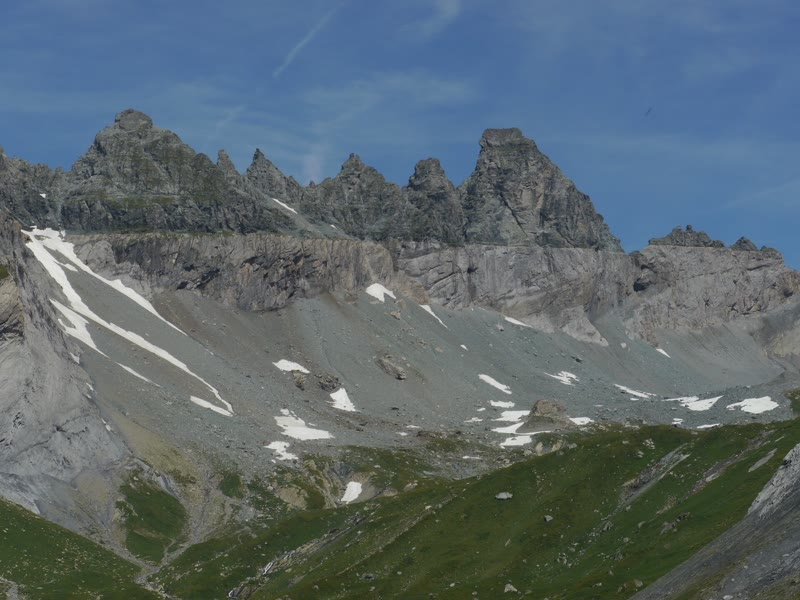
\includegraphics[width=0.5\linewidth]{images/book2/g12-heine-glarus-thrust.jpg}

{\small \omterm{def:g12:mountain-building:thrust}{صدع غلاروس الزاحف} في جبال الألب شرق سويسرا. فالصخور
الداكنة في القمم، التي ترسبت في البرمي، بين نحو 299 و252
مليون سنة مضت، تستقر على صخور أفتح وأحدث بكثير؛ \omterm{def:g12:mountain-building:thrust}{والصدع الزاحف} هو
الحد الحاد بينهما. وقد تحركت الصخور العليا نحو 40 إلى
\qty{50}{km}. الصورة: كريستيان هاينه (\babelsublr{CC~BY-SA~3.0}).}
\end{omfigure}
% ledger: photo:g12-glarus (Verrucano, Permian; displacement 40-50 km, Pfiffner 1985), ics:base.Permian, ics:base.Triassic

\subsection{قياس التقصير}

\omterm{def:g12:mountain-building:fold}{الطيات} \omterm{def:g12:mountain-building:thrust}{والصدوع الزاحفة} كلتاهما تجعل القشرة أقصر في الاتجاه الذي
تُعصر فيه.

\begin{definition}[التقصير]\label{def:g12:mountain-building:shortening}
\emph{تقصير}\index{تقصير} الطبقة هو الكسر من
طولها الذي فقدته: فإذا كان طولها $L_0$ وصارت تمتد الآن على $L$،
\[
  e = \frac{L_0 - L}{L_0}.
\]
\end{definition}

لقياسه، نحتاج إلى الطول الأصلي $L_0$. وفي كثير من \omterm{def:g12:mountain-building:fold}{الطيات} تحتفظ
الطبقات بسمكها وهي تنثني، فتنزلق بعضها فوق بعض كصفحات
كتاب مثني؛ ومثل هذه الطبقة لا تتمطط على امتداد طولها. وهذا
يعطي الطول الأصلي.
% ledger: tulane:fold-geometry (flexural folds keep their thickness)

\begin{proposition}[تقصير طبقة مطوية]\label{prop:g12:mountain-building:shortening}
إذا انطوت طبقة دون أن تتمطط أو تنضغط على امتداد نفسها،
فإن طولها الأصلي $L_0$ هو طولها المقيس على امتداد الطبقة المطوية.
ولطية جناحاها مستقيمان يميلان بزاوية $\theta$،
\[
  e = 1 - \cos\theta .
\]
\end{proposition}

\begin{proof}
بسط الطبقة، دون تمطيطها، يمدّها مستوية
وطولها لم يتغير؛ إذن $L_0$ هو الطول على امتداد الطبقة. وعلى جناح
مستقيم طوله $\ell$ يميل بزاوية $\theta$، تكون المسافة الأفقية المقطوعة
$\ell\cos\theta$ (مثلث قائم). وبجمع كل الأجنحة، تمتد الطبقة التي
طولها $L_0$ على $L = L_0\cos\theta$، و$e = (L_0 - L_0\cos\theta)/L_0 =
1 - \cos\theta$.
\end{proof}

\begin{omfigure}
\begin{tikzpicture}
\begin{axis}[name=sine, x=2.0cm, y=2.0cm, axis lines=none,
  xmin=-0.05, xmax=2.25, ymin=-0.4, ymax=0.8, clip=false]
% computed in figdata/grade-12/fold_shortening.py (part sine: A/lambda = 0.25, e = 31.7 %)
\addplot[omLithSand!80!black, line width=1.6pt] table[x=x, y=y] {figdata/out/grade-12-fold_shortening-sine.dat};
\draw[omThm, line width=1.6pt] (axis cs:0,0.62) -- (axis cs:2.196,0.62);
\draw[black!60, |-|] (axis cs:0,-0.32) -- node[below, font=\scriptsize] {\foreignlanguage{arabic}{$L$ اليوم}} (axis cs:1.5,-0.32);
\node[anchor=south west, font=\scriptsize, omThm] at (axis cs:0,0.64) {\foreignlanguage{arabic}{$L_0$: الطبقة نفسها مبسوطة}};
\end{axis}
\begin{axis}[omrecord, at={(sine.east)}, anchor=west, xshift=1.4cm, width=0.46\linewidth, height=4.6cm,
  xmin=0, xmax=80, ymin=0, ymax=85, xlabel={\foreignlanguage{arabic}{ميل الجناح $\theta$ \babelsublr{(\unit{\degree})}}},
  ylabel={\foreignlanguage{arabic}{التقصير $e$ \babelsublr{(\unit{\percent})}}}, xtick={0,20,...,80}]
% computed in figdata/grade-12/fold_shortening.py (part dip: e = 1 - cos theta)
\addplot[omProp, line width=1pt] table[x=theta, y=e_pct] {figdata/out/grade-12-fold_shortening-dip.dat};
\addplot[only marks, mark=*, mark size=1.6pt, omThm] coordinates {(12,2.185) (30,13.397) (60,50)};
\node[anchor=south, font=\scriptsize, align=center] at (axis cs:12,6) {فاردن\\\babelsublr{\qty{2.2}{\percent}}};
\node[anchor=west, font=\scriptsize] at (axis cs:32,10) {\qty{13}{\percent}};
\node[anchor=south east, font=\scriptsize] at (axis cs:60,51) {\qty{50}{\percent}};
\end{axis}
\end{tikzpicture}

{\small في اليسار: طبقة مطوية تمتد على $L$؛ وإذا بُسطت، دون أن
تتمطط، كان طولها $L_0$ (\omterm{def:g12:mountain-building:fold}{الطيات} هنا ارتفاعها ربع
طول موجتها، و$L$ يساوي \qty{68}{\percent} من $L_0$). في اليمين:
\omterm{def:g12:mountain-building:shortening}{تقصير} \omterm{def:g12:mountain-building:fold}{طية} جناحاها مستقيمان، $1 - \cos\theta$، بدلالة ميل
جناحيها. \omterm{def:g12:mountain-building:fold}{فالطيات} اللطيفة لا تقصّر الطبقة إلا قليلًا جدًا.}
\end{omfigure}
% values: sine_025_e_pct 31.68 (L/L0 = 0.683); varden_e_pct 2.1852; chevron_30 13.397; chevron_60 50 (fold_shortening.py)

\begin{method}[قياس التقصير على مقطع عرضي]\label{met:g12:mountain-building:shortening}
\begin{enumerate}
  \item تحقق من أن المقطع مرسوم بمقياس رسم حقيقي. فإذا كان مقياسه الرأسي
        مُمطَّطًا، كانت الميول والأطوال على امتداد الطبقات أكبر مما ينبغي: فأعد رسمه،
        أو صحح كل ميل أولًا.
  \item اختر حدًا واحدًا بين طبقتين يمكن تتبعه عبر المقطع؛
        وحيث يقطعه صدع، صِل الطرفين المقطوعين كما كانا قبل أن
        يتحرك الصدع.
  \item قس طوله على امتداد الطبقة، $L_0$: تتبعه بخيط،
        أو اجمع قطعًا مستقيمة قصيرة.
  \item قس المسافة الأفقية بين طرفيه، $L$.
  \item احسب $e = (L_0 - L)/L_0$؛ وللأجنحة المستقيمة المعلومة الميل،
        تعطيه $e = 1 - \cos\theta$ مباشرة.
\end{enumerate}
\end{method}

\begin{example}[طيات فاردن]\label{ex:g12:mountain-building:varden}
يميل جناحا \omterm{def:g12:mountain-building:fold}{طيات} فاردن \ang{12}، فقد قُصّر الغطاء الرسوبي بمقدار
$e = 1 - \cos\ang{12} = 1 - 0.978 = 0.022$، أي نحو \qty{2.2}{\percent}:
فشريط من المنطقة عرضه اليوم \qty{10}{km} كان عرضه قبل الطي $10/\cos\ang{12} \approx
\qty{10.22}{km}$. ولو قيس على المقطع A--B كما هو مرسوم، لبدا ميل
الجناحين نحو \ang{28}، لأن المقياس الرأسي
مُمطَّط 2.5 مرة: إذ تُضرب $\tan\theta$ في 2.5، و$\arctan(2.5
\tan\ang{12}) \approx \ang{28}$. ولو أُخذ ذلك على ظاهره، لأعطى
تقصيرًا قدره \qty{12}{\percent}، أي أكثر من خمسة أضعاف القيمة الصحيحة.
\end{example}
% values: varden_e_pct 2.1852, varden_L0_for_10km 10.223 (fold_shortening.py); arctan(2.5 x 0.2126) = 27.98 deg; 1 - cos 27.98 = 0.117

\omterm{def:g12:mountain-building:fold}{الطيات} اللطيفة لا تمتص إلا القليل. أما الحزام المطوي بشدة، الذي يميل جناحاه
\ang{60}، فقد قُصّر إلى النصف؛ \omterm{def:g12:mountain-building:thrust}{وصدع زاحف} واحد يكاد يكون مستويًا
حمل \omterm{def:g12:mountain-building:nappe}{غطاءً تكتونيًا} \qty{40}{km} يمتص \qty{40}{km} من \omterm{def:g12:mountain-building:shortening}{التقصير}، أي ما
يمتصه حزام عريض جدًا من \omterm{def:g12:mountain-building:fold}{الطيات} اللطيفة.

\section{التسمك والنهوض}

\omterm{def:g12:mountain-building:shortening}{التقصير} لا يدمر الصخر. فشريط القشرة الذي يُعصر إلى كسر من
عرضه السابق يحتفظ بحجمه، فلا بد أن يزداد سمكًا: فإذا قُصّرت قشرة
سمكها $H_0$ من عرض $L_0$ إلى $L$ على طول الحزام
كله، احتفظ مقطعها العرضي بمساحته، $H L = H_0 L_0$، ومنه
\[
  H = H_0\,\frac{L_0}{L} = \frac{H_0}{1 - e}.
\]
فالقشرة التي سمكها \qty{35}{km} وقُصّرت بمقدار \qty{50}{\percent} يصير
سمكها \qty{70}{km}. ثم يتكفل \omterm{def:g11:lithosphere-asthenosphere:isostasy}{التوازن الأيزوستاتي} بالباقي: فالقشرة الأسمك تطفو
أعلى، فوق \omterm{def:g12:continental-crust:root}{جذر} أعمق (\cref{prop:g11:lithosphere-asthenosphere:airy}).
ومع نموذج إيري وكثافات ما نعرفه من قبل، فإن القشرة الأسمك بمقدار
$\Delta H$ تقف أعلى بمقدار $\Delta H\,(\rho_m - \rho_c)/\rho_m = \Delta H
\times 550/3380$، أي نحو سدس السمك الزائد؛ والأسداس الخمسة
الأخرى تكوّن \omterm{def:g12:continental-crust:root}{الجذر}. وسمك القشرة من \num{35} إلى \qty{40}{km} بعيدًا عن
الأحزمة الجبلية، ومن 50 إلى \qty{70}{km} تحتها: فكلما علت
الجبال، ازدادت القشرة سمكًا.
% ledger: tulane:roots, cm95:crust, data:prem

هكذا وصل حجر جيري من قاع البحر إلى قمة إيفرست: فقد ترسب على
قاع بحر، ثم حُمل شمالًا مع الهند، وكُدّس في الصفائح
الزاحفة للهيمالايا، ورُفع كلما تسمكت القشرة تحته
وارتفعت. وتُسمّى هذه الحركة الرأسية للقشرة النهوض.
% ledger: sakai05:summit, sakai05:stacking, tulane:roots (uplift), usgs:himalaya-collision

\section{سلسلتان}

\subsection{الهيمالايا}

تمتد الهيمالايا \qty{2900}{km} على امتداد الحدود بين الهند
والتبت. فقبل نحو 80 مليون سنة كانت الهند تقع على بعد نحو \qty{6400}{km} جنوب
آسيا، عبر محيط، وتتحرك شمالًا بنحو \qty{9}{cm} في السنة؛ ثم التقت
آسيا بين 40 و50 مليون سنة مضت، فتباطأ عندئذ تقدمها نحو الشمال.
وتُظهر إعادات بناء الصفائح هذه الرحلة بالتفصيل: فهي، وقد بُنيت من أنواع كثيرة
من الأدلة، منها مسارات النقاط الساخنة
(\cref{ch:g11:plate-motions})، تعيد الصفائح إلى الوراء في الزمن خطوة
خطوة.
% ledger: usgs:himalaya-collision, muller19:frame, muller22:frame

\begin{omfigure}
\begin{tikzpicture}
\begin{axis}[omrecord, omage, name=lat, width=0.5\linewidth, height=5.2cm,
  xmin=0, xmax=100, ymin=-45, ymax=35, xlabel={\foreignlanguage{arabic}{العمر \babelsublr{(\unit{Ma})}}}, ylabel={\foreignlanguage{arabic}{خط العرض \babelsublr{(\unit{\degree})}}},
  xtick={0,20,...,100}, ytick={-40,-20,...,40},
  legend style={font=\scriptsize, at={(0.98,0.03)}, anchor=south east, fill=white}]
% computed in figdata/grade-12/india_drift.py (part lat; GPlates Web Service, MULLER2022 and MULLER2019)
\fill[omThm!12] (axis cs:40,-45) rectangle (axis cs:50,35);
\addplot[omThm, line width=1.1pt] table[x=age, y=m22_india] {figdata/out/grade-12-india_drift-lat.dat};
\addplot[omThm, dashed, line width=0.8pt] table[x=age, y=m19_india] {figdata/out/grade-12-india_drift-lat.dat};
\addplot[omDef, line width=1.1pt] table[x=age, y=m22_lhasa] {figdata/out/grade-12-india_drift-lat.dat};
\addplot[black!50, line width=0.4pt, forget plot] coordinates {(0,0) (100,0)};
\legend{{\foreignlanguage{arabic}{وسط الهند، نموذج 2022}}, {\foreignlanguage{arabic}{وسط الهند، نموذج 2019}}, {\foreignlanguage{arabic}{لاسا، نموذج 2022}}}
\end{axis}
\begin{axis}[omrecord, omage, at={(lat.east)}, anchor=west, xshift=1.9cm, width=0.42\linewidth, height=5.2cm,
  xmin=0, xmax=100, ymin=0, ymax=160, xlabel={\foreignlanguage{arabic}{العمر \babelsublr{(\unit{Ma})}}},
  ylabel={\foreignlanguage{arabic}{السرعة نحو الشمال \babelsublr{(\unit{mm/yr})}}}, xtick={0,20,...,100}]
% computed in figdata/grade-12/india_drift.py (part steps: 5-Myr steps)
\fill[omThm!12] (axis cs:40,0) rectangle (axis cs:50,160);
\addplot[omThm, line width=1pt] table[x=age, y=m22] {figdata/out/grade-12-india_drift-steps.dat};
\addplot[omThm, dashed, line width=0.7pt] table[x=age, y=m19] {figdata/out/grade-12-india_drift-steps.dat};
\end{axis}
\end{tikzpicture}

{\small في اليسار: خط عرض نقطة في وسط الهند (\ang{78} شرقًا،
\ang{20} شمالًا اليوم) وخط عرض لاسا، شمال \omterm{def:g12:mountain-building:suture}{الدرز}، خلال آخر 100
مليون سنة، في إعادتي بناء منشورتين للصفائح (2022 و2019).
في اليمين: سرعة الهند نحو الشمال في كل خطوة من 5 ملايين سنة. والشريط
المظلل يحدد الفترة من 40 إلى 50 مليون سنة مضت. البيانات: ر.~د.~مولر وزملاؤه
(2019، 2022)، محسوبة بخدمة \babelsublr{GPlates} على الويب.}
\end{omfigure}
% ledger: data:b2-gws-india, muller22:frame, muller19:frame; values: speed_65_50 128.5, speed_40_0 40.06, fastest 145.8 (50-55 Ma) (india_drift.py)

تتفق إعادتا البناء في حدود بضع درجات. فبين 65 و50 مليون
سنة مضت تحركت الهند شمالًا بنحو \qty{13}{cm} في السنة؛ وبين 50 و40
مليون سنة مضت انخفضت سرعتها،
ومنذ 40 مليون سنة تتحرك بنحو \qty{4}{cm} في السنة، أي أقل
من ثلث تلك السرعة. أما لاسا، على الجانب الآسيوي، فقد تحركت شمالًا أيضًا، لكن
ببطء أكبر بكثير.
% values: speed_65_50 128.5 mm/yr, speed_40_0 40.06 mm/yr, slowdown_ratio 0.312 (india_drift.py)

\begin{example}[سرعة الهند]\label{ex:g12:mountain-building:india}
في إعادة بناء 2022، كان وسط الهند عند \ang{12.10} جنوبًا قبل 60 مليون
سنة وعند \ang{0.68} جنوبًا قبل 50 مليون سنة. ودرجة العرض الواحدة تساوي
$2\pi R/360 = 2\pi \times \qty{6371}{km}/360 \approx \qty{111.2}{km}$. فقد
تحركت الهند شمالًا مسافة $(12.10 - 0.68) \times 111.2 \approx \qty{1270}{km}$ في 10
ملايين سنة: أي \qty{127}{km} في كل مليون سنة، وهذا يعني $\qty{127e6}{mm} /
\num{e6}\text{ سنة} = \qty{127}{mm}$، أي نحو \qty{13}{cm}، في السنة.
\end{example}
% ledger: data:b2-gws-india, earth:Rmean; values: lat 60 Ma -12.0964, 50 Ma -0.6801 (india_drift-lat)

يُقرأ التباطؤ علامةً على الاصطدام: \omterm{def:g12:continental-crust:continental-crust}{فالقشرة القارية}
الواصلة إلى الخندق لم تستطع أن تغوص، فأُعيقت الهند. والتاريخ الدقيق للتماس الأول لا يزال موضع نقاش: فالتقديرات
تتراوح بين نحو 60 و54 مليون سنة مضت، ويرى بعض الجيولوجيين أن
الهند التقت أولًا سلسلة من الجزر البركانية ولم تبلغ آسيا نفسها إلا
قبل نحو 34 مليون سنة. ولم تتوقف الهند: فأقطاب دوران
صفائح اليوم تحركها نحو أوراسيا بنحو \qty{4.5}{cm} في السنة عبر
الهيمالايا (\cref{ch:g11:plate-motions})، والضغط يعصر أجزاء من
آسيا نحو الشرق.
% ledger: usgs:himalaya-collision, najman21:collision-age; values: today_in_eu_speed 44.99 mm/yr (india_drift.py, from nnr56:poles)

شمال الهيمالايا، تقف هضبة التبت على ارتفاع نحو \qty{4600}{m} في
المتوسط، فوق قشرة سمكها نحو \qty{70}{km}
(\cref{ch:g11:lithosphere-asthenosphere}). وبين الهند والتبت يقع
\omterm{def:g12:mountain-building:suture}{درز} السند--تسانغبو بأوفيوليتاته؛ وجنوبه، تتكون الهيمالايا
في معظمها من رسوبيات ترسبت على الحافة الشمالية للهند، ثم كُدّست
وطُويت وتصدعت، ومنها حجر قمة إيفرست الجيري.
% ledger: karplus:tibet-moho, liu20:itsz, sakai05:stacking, sakai05:summit; Book 1: usgs:himalaya (Tibetan Plateau about 4600 m)

\subsection{الألب، وحزام كامل}

للألب تاريخ مماثل على نطاق أصغر: فقد ارتفعت حيث اصطدمت إفريقيا
بأوروبا. وهي أيضًا تحوي \omterm{def:g12:mountain-building:ophiolite}{أوفيوليتات}، \omterm{def:g12:mountain-building:thrust}{وصدوعًا زاحفة} كبيرة: فعند
\omterm{def:g12:mountain-building:thrust}{صدع غلاروس الزاحف}، حُملت صخور برمية فوق صخور أحدث منها بكثير.
والألب والهيمالايا ينتميان إلى حزام جبلي واحد طويل، يمر عبر
زاغروس في إيران، حيث اصطدمت إفريقيا والهند بأوراسيا.
% ledger: earle:collision, photo:g12-glarus

\begin{omfigure}
\begin{tikzpicture}
\begin{axis}[axis equal image, xmin=-12, xmax=105, ymin=18, ymax=52, width=\linewidth,
  tick label style={font=\scriptsize}, xtick={0,30,60,90}, ytick={20,30,40,50},
  xticklabel={$\pgfmathprintnumber{\tick}^\circ$}, yticklabel={$\pgfmathprintnumber{\tick}^\circ$},
  axis background/.style={fill=omSea}, legend columns=3,
  legend style={font=\scriptsize, at={(0.5,-0.12)}, anchor=north, /tikz/every even column/.append style={column sep=5pt}}]
\addplot[fill=omLithAlluv, draw=black!45, line width=0.2pt, forget plot] table {figdata/out/shared-geo-land.dat};
% computed in figdata/grade-12/alpine_belt.py; ledger: data:etopo1, data:usgs-comcat
\addplot[only marks, mark=square*, mark size=1.15pt, omLithSand!85!black] table[x=lon, y=lat] {figdata/out/grade-12-alpine_belt-high.dat};
\addplot[only marks, mark=square*, mark size=1.15pt, omThm!75!black] table[x=lon, y=lat] {figdata/out/grade-12-alpine_belt-higher.dat};
\addplot[only marks, mark=*, mark size=0.7pt, black] table[x=lon, y=lat] {figdata/out/grade-12-alpine_belt-quakes.dat};
\addplot[omDef, line width=0.9pt, forget plot] table {figdata/out/shared-geo-school-collision.dat};
\addplot[black!70, line width=0.5pt, forget plot] table {figdata/out/shared-geo-school-subduction.dat};
\legend{{\foreignlanguage{arabic}{أعلى من \babelsublr{\qty{1500}{m}}}}, {\foreignlanguage{arabic}{أعلى من \babelsublr{\qty{3500}{m}}}}, {\foreignlanguage{arabic}{زلزال قدره 6 أو أكثر}}}
\coordinate (alps) at (axis cs:9,48);
\coordinate (zagros) at (axis cs:46,23.5);
\coordinate (zagrosbelt) at (axis cs:50.5,31.5);
\coordinate (himal) at (axis cs:84,24);
\coordinate (tibet) at (axis cs:88,33);
\coordinate (arrA) at (axis cs:77,19.5);
\coordinate (arrB) at (axis cs:79.2,25);
\end{axis}
% labels drawn after the axis, so that no earthquake dot covers them
\node[font=\scriptsize, fill=white, inner sep=1pt, anchor=south] at (alps) {الألب};
\draw[black!60, line width=0.4pt] (zagros) -- (zagrosbelt);
\node[font=\scriptsize, fill=white, inner sep=1pt] at (zagros) {زاغروس};
\node[font=\scriptsize, fill=white, inner sep=1pt, anchor=west] at (himal) {الهيمالايا};
\node[font=\scriptsize, fill=white, inner sep=1pt] at (tibet) {هضبة التبت};
\draw[-{Stealth[length=2mm]}, line width=1pt, omProp] (arrA) -- (arrB);
\end{tikzpicture}

{\small حزام الجبال الفتية من الأطلسي إلى التبت: الأراضي المرتفعة
(كل مربع خلية من درجة واحدة)، والزلازل الضحلة التي قدرها 6 أو أكثر
من 1976 إلى 2025 (الأقل عمقًا من \qty{70}{km})، وحدود
الاصطدام بين الصفائح (الخط الأزرق). ويبين السهم حركة الهند
نحو أوراسيا. البيانات: \babelsublr{ETOPO1}، وفهرس الزلازل لهيئة المسح الجيولوجي الأمريكية، وحدود الصفائح من
بيرد (2003)، واليابسة من \babelsublr{Natural Earth}.}
\end{omfigure}
% ledger: data:etopo1, data:usgs-comcat, data:pb2002, data:ne-land; values: n_quakes 398 (alpine_belt.py)

الأراضي المرتفعة والزلازل تتبع الشريط الضيق نفسه. فالاصطدام
لم ينتهِ: والزلازل تُظهر أن القشرة لا تزال تنكسر
على امتداد الحزام كله، وأن الجبال لا تزال تُبنى.

\section{تمارين}

\begin{exercise}[$\star$]\label{exo:g12:mountain-building:1}
طابق كل مصطلح مع وصفه: \omterm{def:g12:mountain-building:fold}{الطية المحدبة}، \omterm{def:g12:mountain-building:fold}{الطية المقعرة}، \omterm{def:g12:mountain-building:thrust}{الصدع الزاحف}، \omterm{def:g12:mountain-building:nappe}{الغطاء التكتوني}،
\omterm{def:g12:mountain-building:suture}{الدرز}، \omterm{def:g12:mountain-building:ophiolite}{الأوفيوليت}. (أ) \omterm{def:g12:mountain-building:thrust}{صدع معكوس} ميله خفيف؛ (ب) قطعة من
قاع المحيط توجد على اليابسة؛ (ج) \omterm{def:g12:mountain-building:fold}{طية} يميل جناحاها نحو محورها؛
(د) الخط الذي التحمت عنده قارتان؛ (ه) \omterm{def:g12:mountain-building:fold}{طية} يميل جناحاها
بعيدًا عن محورها؛ (و) صفيحة صخرية كبيرة حُملت بعيدًا على امتداد \omterm{def:g12:mountain-building:thrust}{صدع زاحف}.
\end{exercise}

\begin{exercise}[$\star$]\label{exo:g12:mountain-building:2}
على جانبي وادٍ، تميل الطبقات في الجانب الغربي \ang{20} نحو الغرب
وتميل التي في الجانب الشرقي \ang{20} نحو الشرق. (1) هل \omterm{def:g12:mountain-building:fold}{الطية} التي بينهما
\omterm{def:g12:mountain-building:fold}{طية محدبة} أم مقعرة؟ (2) بعد التعرية، هل توجد أقدم الطبقات أم أحدثها
على امتداد محورها؟ (3) هل يجب أن يقع الوادي فوق \omterm{def:g12:mountain-building:fold}{طية مقعرة}؟
\end{exercise}

\begin{exercise}[$\star$]\label{exo:g12:mountain-building:3}
طبقة مطوية جناحاها مستقيمان يميلان \ang{30}. (1) احسب
تقصيرها. (2) تمتد اليوم على \qty{6.0}{km}. فكم كان طولها؟
\end{exercise}

\begin{exercise}[$\star$]\label{exo:g12:mountain-building:4}
(1) على امتداد صدع، تحركت الكتلة التي فوق مستوى الصدع إلى الأسفل. فهل هو
\omterm{def:g11:ocean-ridges:normal-fault}{صدع عادي} أم معكوس، وهل تمططت القشرة أم عُصرت؟
(2) \omterm{def:g12:mountain-building:thrust}{صدع معكوس} يميل \ang{25}: هل هو \omterm{def:g12:mountain-building:thrust}{صدع زاحف}؟
\end{exercise}

\begin{exercise}[$\star$]\label{exo:g12:mountain-building:5}
(1) رتّب صخور \omterm{def:g12:mountain-building:ophiolite}{الأوفيوليت} هذه من الأعلى إلى الأسفل: \omterm{def:g11:ocean-ridges:gabbro}{الغابرو}،
والرسوبيات البحرية، \omterm{def:g11:ocean-ridges:peridotite}{والبيريدوتيت}، والبازلت الوسائدي، \omterm{def:g11:igneous-rocks:intrusion}{والقواطع} المتراصة. (2) لماذا يدل
البازلت الوسائدي على أن الصخر تكوّن تحت الماء؟ (3) لماذا توجد
\omterm{def:g12:mountain-building:ophiolite}{الأوفيوليتات} على امتداد الدروز؟
\end{exercise}

\begin{exercise}[$\star\star$]\label{exo:g12:mountain-building:6}
على مقطع عرضي بمقياس رسم حقيقي، يُتتبع حد حجر رملي عبر أربع
قطع مستقيمة أطوالها \qty{2.1}{km} و\qty{1.8}{km} و\qty{2.4}{km}
و\qty{1.6}{km}؛ والمسافة بين طرفيه \qty{6.0}{km}. (1) احسب
\omterm{def:g12:mountain-building:shortening}{التقصير}. (2) إذا كانت الأجنحة الأربعة كلها تميل بالزاوية نفسها، فما هي؟
\end{exercise}

\begin{exercise}[$\star\star$]\label{exo:g12:mountain-building:7}
تحركت الكتلة العليا \omterm{def:g12:mountain-building:thrust}{لصدع زاحف} يميل \ang{10} مسافة \qty{45}{km} على امتداد
مستوى الصدع. (1) كم تحركت أفقيًا؟ (2) كم
ارتفعت؟ (3) ما عرض حزام من \omterm{def:g12:mountain-building:fold}{الطيات} يميل جناحاها \ang{12} يمتص
\omterm{def:g12:mountain-building:shortening}{التقصير} الأفقي نفسه؟
\end{exercise}

\begin{exercise}[$\star\star$]\label{exo:g12:mountain-building:8}
على امتداد \omterm{def:g12:mountain-building:thrust}{صدع ماكونيل الزاحف}، يستقر حجر جيري عمره نحو 500 مليون سنة على
حجر طيني عمره نحو 75 مليون سنة. (1) أي مبدأ من مبادئ التأريخ النسبي
يضلل جيولوجيًا يتجاهل الصدع؟ (2) بكم تزيد أقدمية
الصخر الأعلى؟ (3) سمك الصفيحة الزاحفة نحو \qty{800}{m} وقد تحركت
\qty{40}{km}: فكم ضعفًا من سمكها هذه المسافة؟
\end{exercise}

\begin{exercise}[$\star\star$]\label{exo:g12:mountain-building:9}
في إعادة بناء 2022، كان وسط الهند عند \ang{30.23} جنوبًا قبل 80 مليون
سنة وعند \ang{19.38} جنوبًا قبل 66 مليون سنة. (1) ما المسافة التي
تحركها نحو الشمال؟ (2) بأي سرعة متوسطة، بوحدة \unit{cm} في السنة؟ (3) قارنها
بملخص هيئة المسح الجيولوجي الأمريكية، نحو \qty{9}{m} في القرن.
\end{exercise}

\begin{exercise}[$\star\star$]\label{exo:g12:mountain-building:10}
قشرة سمكها \qty{35}{km} قُصّرت بمقدار \qty{40}{\percent} عبر
حزام كامل. (1) كم يصير سمكها؟ (2) مع $\rho_c =
\qty{2830}{kg/m^3}$ و$\rho_m = \qty{3380}{kg/m^3}$، بكم ترتفع
أكثر، وما عمق \omterm{def:g12:continental-crust:root}{جذرها} الإضافي؟
\end{exercise}

\begin{exercise}[$\star\star$]\label{exo:g12:mountain-building:11}
على مقطع رُسم بمقياس رأسي مُمطَّط 3 مرات، يبدو أن جناحًا
يميل \ang{40}. (1) ما ميله الحقيقي؟ (2) احسب \omterm{def:g12:mountain-building:shortening}{التقصير} من
الميل الحقيقي ومن الميل المقروء على الرسم. (3) لماذا يجب أن تُرسم المقاطع المستعملة
لقياس \omterm{def:g12:mountain-building:shortening}{التقصير} بمقياس رسم حقيقي؟
\end{exercise}

\begin{exercise}[$\star\star\star$]\label{exo:g12:mountain-building:12}
\omterm{def:g12:mountain-building:fold}{الطيات} المستديرة المرسومة في هذا الفصل، التي ارتفاعها ربع
طول موجتها، تقصيرها \qty{31.7}{\percent}؛ وأشد ميل فيها
نحو \ang{57.5}. (1) طبقة مطوية على هذا النحو تمتد على \qty{10}{km}: فكم
كان طولها؟ (2) احسب \omterm{def:g12:mountain-building:shortening}{تقصير} \omterm{def:g12:mountain-building:fold}{طية} جناحاها مستقيمان عند
\ang{57.5}. (3) فسّر لماذا تقصّر \omterm{def:g12:mountain-building:fold}{الطية} ذات الجناحين المستقيمين أكثر لأشد
ميل نفسه.
\end{exercise}

\begin{exercise}[$\star\star\star$]\label{exo:g12:mountain-building:13}
شمال الهيمالايا، عند \ang{85} شرقًا و\ang{28} شمالًا، تعطي أقطاب الدوران الهند
سرعة بالنسبة إلى أوراسيا قدرها \qty{16.6}{mm/yr} نحو الشرق
و\qty{41.8}{mm/yr} نحو الشمال. وخلال آخر 5 ملايين سنة، تعطي إعادة بناء 2022
وسط الهند سرعة نحو الشمال تزيد بمقدار \qty{23.5}{mm/yr}
على سرعة لاسا. (1) جد سرعة الهند بالنسبة إلى
أوراسيا. (2) بافتراض أن المركبتين الشماليتين قابلتان للمقارنة، فكم يبقى من \omterm{def:g12:mountain-building:shortening}{التقصير}
الشمالي--الجنوبي في كل مليون سنة للمنطقة الواقعة شمال
لاسا؟ (3) أين في الفصل علامة على أن هذه المنطقة تتشوه؟
\end{exercise}

\begin{exercise}[$\star\star\star$]\label{exo:g12:mountain-building:14}
في الألب، حُمل \omterm{def:g12:mountain-building:nappe}{غطاء تكتوني} \qty{45}{km} على امتداد \omterm{def:g12:mountain-building:thrust}{صدع زاحف} ميله
قريب من الصفر. (1) ما \omterm{def:g12:mountain-building:shortening}{التقصير} الذي امتصه ذلك الصدع؟ (2) ما العرض،
قبل الطي، من غطاء رسوبي مطوي مثل غطاء تلال فاردن (أجنحة
\ang{12}) الذي يمتص \omterm{def:g12:mountain-building:shortening}{التقصير} نفسه؟ (3) ماذا يُظهر ذلك عن
كيفية امتصاص الأحزمة الجبلية للتقاربات الكبيرة؟
\end{exercise}

\begin{exercise}[$\star\star\star$]\label{exo:g12:mountain-building:15}
ترسب حجر قمة إيفرست الجيري على قاع بحر، أدنى من مستوى سطح البحر ولو
قليلًا، وهو يقف اليوم على ارتفاع \qty{8848.86}{m}. (1) باعتبار
أن الاصطدام بدأ قبل 50 مليون سنة، ما أدنى معدل متوسط
للنهوض، بوحدة \unit{mm} في السنة؟ (2) قارنه بسرعة الهند منذ
40 مليون سنة، نحو \qty{40}{mm} في السنة. (3) لماذا يُرجَّح أن يكون نهوض
الصخر أكبر من ارتفاعه الحالي؟
\end{exercise}

\begin{problem}[{مسألة نهاية الأسبوع --- رحلة الهند}]
\label{pb:g12:mountain-building:1}
% ledger: data:b2-gws-india, earth:Rmean, usgs:himalaya-collision, tulane:roots, cm95:crust, data:prem, karplus:tibet-moho; Book 1: usgs:himalaya (4600 m)
% values: india_drift-lat (MULLER2022, rounded to 0.01 deg); north_since_66_km 4378.7; converge_since_50 1354; gap_0 1073
يعطي الجدول خط عرض نقطة في وسط الهند وخط عرض لاسا،
شمال \omterm{def:g12:mountain-building:suture}{الدرز}، في إعادة بناء الصفائح لعام 2022 (السالب = جنوب).
خذ درجة العرض الواحدة \qty{111.2}{km}، وخذ \qty{1}{km} في كل مليون
سنة على أنه \qty{1}{mm} في السنة.

\begin{center}
\small
\begin{tabular}{|l|c|c|c|c|c|c|c|c|c|}
\hline
العمر (\unit{Ma}) & 80 & 66 & 60 & 55 & 50 & 45 & 40 & 20 & 0 \\ \hline
الهند (\unit{\degree}) & $-30.23$ & $-19.38$ & $-12.10$ & $-7.24$ & $-0.68$ & 3.30 & 5.59 & 13.40 & 20.00 \\ \hline
لاسا (\unit{\degree}) & & 19.48 & & & 21.15 & & & & 29.65 \\ \hline
\end{tabular}
\end{center}

\medskip
\noindent\textbf{الجزء الأول --- خطوط العرض والسرعات.}
\begin{enumerate}
  \item تحقق من القيمة \qty{111.2}{km} لدرجة واحدة، مع $R =
        \qty{6371}{km}$.
  \item متى عبر وسط الهند خط الاستواء؟
  \item ما المسافة التي تحركتها الهند نحو الشمال من 66 إلى 50 مليون سنة مضت؟
  \item بأي سرعة متوسطة؟
  \item احسب سرعتها في كل خطوة من 66 إلى 40 مليون سنة مضت (من 66
        إلى 60، ومن 60 إلى 55، وهكذا). في أي خطوة كانت أسرع؟
\end{enumerate}

\medskip
\noindent\textbf{الجزء الثاني --- التباطؤ.}
\begin{enumerate}[resume]
  \item احسب سرعة الهند المتوسطة من 40 مليون سنة مضت إلى اليوم.
  \item ما الكسر الذي يمثله ذلك من سرعتها من 66 إلى 50 مليون سنة مضت؟
  \item بين أي تاريخين من تواريخ الجدول انخفضت السرعة أكثر؟
  \item لماذا يبطئ الاصطدام الصفيحة؟
  \item ما المسافة التي تحركتها الهند نحو الشمال من 50 مليون سنة مضت إلى اليوم؟
\end{enumerate}

\medskip
\noindent\textbf{الجزء الثالث --- التقارب الممتص.}
\begin{enumerate}[resume]
  \item ما المسافة التي تحركتها لاسا نحو الشمال من 50 مليون سنة مضت إلى اليوم؟
  \item بكم تقلصت المسافة الشمالية--الجنوبية بين وسط الهند
        ولاسا منذ 50 مليون سنة؟
  \item ما هذه المسافة اليوم، وما كانت قبل 50 مليون سنة؟
  \item افترض أن هذا التقارب كله امتصه \omterm{def:g12:mountain-building:shortening}{تقصير}
        القشرة بين النقطتين. فما \omterm{def:g12:mountain-building:shortening}{التقصير} $e$؟
  \item سمّ نوعي البنى اللذين يمتصان مثل هذا \omterm{def:g12:mountain-building:shortening}{التقصير}.
\end{enumerate}

\medskip
\noindent\textbf{الجزء الرابع --- القشرة المُسمَّكة.}
\begin{enumerate}[resume]
  \item إذا كان سمك تلك القشرة \qty{35}{km} قبل 50 مليون سنة، فكم
        سيكون سمكها الآن، مع احتفاظها بمقطعها العرضي؟
  \item مع $\rho_c = \qty{2830}{kg/m^3}$ و$\rho_m = \qty{3380}{kg/m^3}$،
        كم سترتفع فوق مستواها السابق؟
  \item تقف هضبة التبت على ارتفاع نحو \qty{4600}{m}، فوق قشرة
        سمكها نحو \qty{70}{km}. فأي سمك للقشرة يعطيه نموذج إيري
        لارتفاع \qty{4600}{m}؟
  \item اذكر سببًا واحدًا يجعل النموذج البسيط في السؤال 16 يبالغ في تقدير
        التسمك.
  \item بجمع مسافتي السؤالين 3 و10، ما المسافة التي قطعتها الهند
        نحو الشمال منذ نهاية الطباشيري، قبل 66 مليون
        سنة؟
\end{enumerate}
\end{problem}
